\section{实验结果}
纬度校正结果如下图:
\begin{figure}[H]
	\centering
	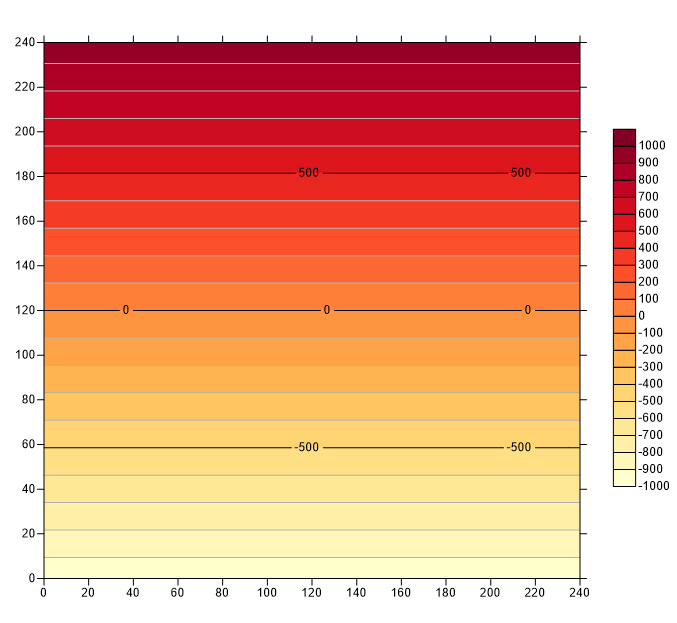
\includegraphics[scale = 0.85]{figures/g_phi.png}
	\caption{维度矫正结果}
\end{figure}

中间层校正结果如下图:
\begin{figure}[H]
	\centering
	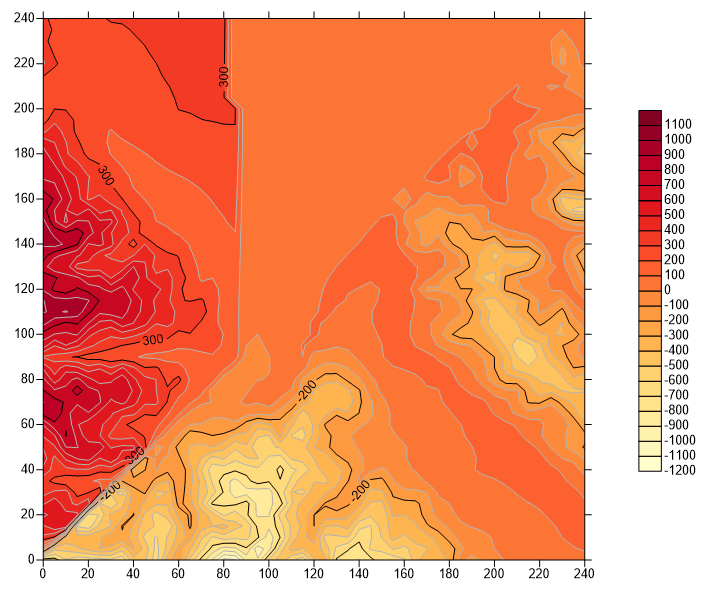
\includegraphics[scale = 0.85]{figures/g_m.png}
	\caption{中间层矫正结果}
\end{figure}

高度校正结果如下图:
\begin{figure}[H]
	\centering
	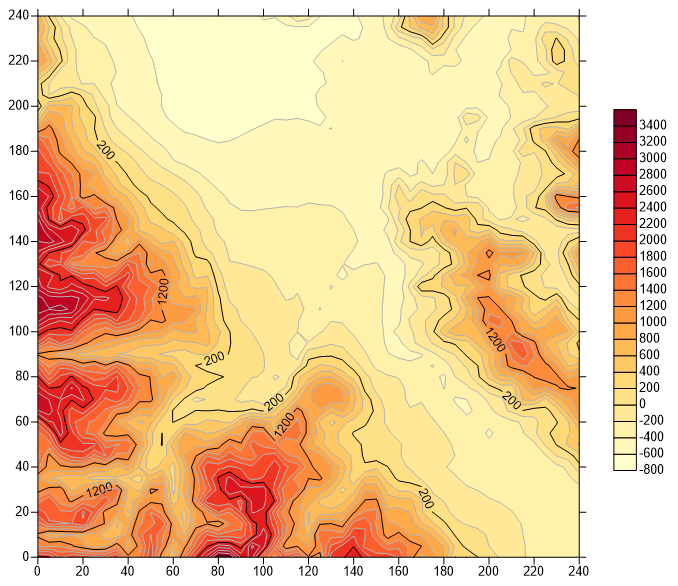
\includegraphics[scale = 0.85]{figures/g_h.png}
	\caption{高度校正结果}
\end{figure}

本次实验处理了布格重力误差中的纬度异常、高度异常、中间层异常,并未处理地形校正一项。在处理地形校正时,应当先确定方形区域的划分范围,而且求取各个区域中的$K_{ij}$值,从而求得地形校正值。值得注意的是,在纬度校正中,距离$D$表示的是纬向距离,也就是$y$坐标上的距离。

做好重力数据预处理,下一步就是要对重力异常进行分析,求一次导等工作,分析重力异常的变化趋势。